% Redefining the chapter Heading
\makeatletter
\def\@makechapterhead#1{%
  \vspace*{50\p@}%
  {\parindent \z@ \raggedright \normalfont
        %\huge\bfseries \@chapapp\space \thechapter
        \Huge\bfseries \thechapter.\space Annex%
        %\par\nobreak
        %\vskip 20\p@
        \vskip 40\p@
  }}
\makeatother

\chapter{Annex}\label{chap:annex}
This annex contains results and experiments that we consider secondary in relation to the main content. \Cref{sec:dconvexity,sec:annex_dconvex_pbox} presents additional results concerning copulas presented in \Cref{sec:copulas} and used in \Cref{subsec:pboxes,subsec:pboxes}. \Cref{sec:median_filtering} presents results on the median filter used in \Cref{sec:coherence_disparity_intervals}. \Cref{sec:ablation_study} contains ablation studies of the method presented in \Cref{chap:epistemic_uncertainty}. 


\section{Directional Convexity/Concavity for Copulas}\label{sec:dconvexity}
This section will investigate a property shared by some copulas called directional convexity/concavity. This is a theoretical contribution, as we do not exploit them in the applications to stereophotogrammetry in \Cref{chap:propagating,chap:epistemic_uncertainty}. However, we will see that those properties are shared by many common families of copulas. The main result of this section is \cref{eq:convex_diff_hvol}, which was used to prove a specific relationship between multivariate uncertainty models in \Cref{subsec:pboxes,subsec:multiple_models}.

\begin{definition}[D-convexity, D-concavity]\label{def:convex}
    A copula $C$ is called directionally convex (D-convex) \cite{alvoni_dierent_2007} if for every $(u_1 \enum u_n)\in[0,1]^n$, $(v_1\enum v_n)\in[0,1]^n$, $i\in\opi1,n\cli$ and $t\in[0,1]$ it verifies:
    \begin{align}
        C(u_1\enum tu_i+(1-t)v_i\enum u_n) ~\leqslant~&t\cdot C(u_1\enum u_i\enum u_n)\nonumber\\
        &+ (1-t)\cdot C(u_1\enum v_i\enum u_n)\label{eq:convex_copula}
    \end{align}
    In other words, the copula is convex when fixing all but one of its variables. A copula is called directionally concave (D-concave) if the inequality is reversed.
\end{definition}

D-convexity/D-concavity is quite common in known families of copulas. The following paragraphs detail this property for copulas presented in \Cref{tab:family_of_copula}, in the case $n=2$.
As the copulas presented are symmetric regarding their variables, D-convexity/D-concavity is only detailed for $u_1$. We assume that \( \theta \) always belong to the domain of definition detailed in \Cref{tab:family_of_copula}, and that \(u_1, u_2\) are in \([0, 1]\). Regarding the Clayton and Gumbel families, the copula is defined by continuous extension in cases $u_1=0$ and $u_2=0$. Finally, if the restriction of a copula $C$ to one of its variable $u_i$ is twice differentiable, then proving its D-convexity for this variable can be done by proving that $\dfrac{\partial^2 C}{\partial {u_i}^2}\geqslant 0$.
\begin{description}
    \item[Ali-Mikhail-Haq copula] This copula is twice differentiable, and its second order partial derivative is
    $$\frac{\partial^2 C}{\partial {u_1}^2}=u_2(1-\theta(1-u_2))\frac{-2\theta(1-u_2)}{(1-\theta(1-u_1)(1-u_2))^3}$$
    Thus the Ali-Mikhail-Haq copula is D-convex for $\theta\in[-1,0]$ and D-concave for $\theta\in[0,1)$.
    \item[Clayton copula] This copula is not always differentiable on all of its domain, depending on which value is retained by the maximum function. It is however continuous as it is the maximum of two continuous function. For convenience, we work with $(u_1, u_2)$ in $\mathbb{I}^2$, where $\mathbb{I}$ is the open unit interval (the closed unit interval is then covered by continuity). Let $u_2\in\mathbb{I}$. We split the possible range $\mathbb{I}$ of $u_1$ in two:
\begin{itemize}
    \item the first domain $\mathcal{D}_1^{\theta,u_2}$ is where $u_1^{-\theta}+u_2^{-\theta}-1\leqslant0$, and thus $C(u_1, u_2)=0$. Here, $\frac{\partial^2 C}{\partial {u_1}^2}=0$ and the copula is both D-convex and D-concave.
    \item the second domain $\mathcal{D}_2^{\theta,u_2}$ is where $u_1^{-\theta}+u_2^{-\theta}-1>0$ and thus $C(u_1, u_2)\geqslant0$. Here it holds that
    $$\frac{\partial^2 C}{\partial {u_1}^2}=(1+\theta)(1-u_2^{-\theta})u_1^{-2-\theta}(u_1^{-\theta}+u_2^{-\theta}-1)^{-2-\frac{1}{\theta}}$$
    Because of the definition of $\mathcal{D}_2^{\theta,u_2}$, the sign of $\frac{\partial^2 C}{\partial {u_1}^2}$ on $\mathcal{D}_2^{\theta,u_2}$ is that of $1-u_2^{-\theta}$.
\end{itemize}

If $\theta>0$, then $D^\theta_2=\mathbb{I}$ and $\frac{\partial^2 C}{\partial {u_1}^2}\leqslant0$ which means that the copula is D-concave on all of its domain.

The case where $\theta<0$ is less straightforward. In that case, $\frac{\partial^2 C}{\partial {u_1}^2}\geqslant0$ on $\mathcal{D}_2^{\theta,u_2}$. The restrictions of the copula to $\mathcal{D}_1^{\theta,u_2}$ and $\mathcal{D}_2^{\theta,u_2}$ are both D-convex, but we need to prove that it is still true on their union. Let $u_1\in\mathcal{D}_1^{\theta,u_2}$, $v_1\in\mathcal{D}_2^{\theta,u_2}$ and $t\in[0,1]$. We note $w_1=(1-u_2^{-\theta})^{-\frac{1}{\theta}}$, such that $\mathcal{D}_1^{\theta,u_2}=]0,w_1]$ and $\mathcal{D}_2^{\theta,u_2}=]w_1, 1[$. By continuity, $C$ is D-convex on $\mathcal{D}_2^{\theta,u_2}\bigcup\{w_1\}$. Because $u_1,w_1\in \mathcal{D}_1^{\theta,u_2}$, it holds that:
    \begin{eqnarray*}
        tC(u_1,~u_2)+(1-t)C(v_1,~u_2) &=& tC(w_1,~u_2)+(1-t)C(v_1,~u_2)\\
        &\geqslant& C(tw_1+(1-t)v_1,~u_2)\\
        &&\text{by convexity of $C$ on $\mathcal{D}_2^{\theta,u_2}\bigcup\{w_1\}$}\\
        &\geqslant& C(tu_1+(1-t)v_1,~u_2)\\
        && \text{because $C$ is component-wise increasing}
    \end{eqnarray*}
which, by definition \ref{def:convex}, proves that $C$ is D-convex on $\mathcal{D}_1^{\theta,u_2}\bigcup \mathcal{D}_2^{\theta,u_2}$. By continuity, $C$ is D-convex on all of its domain.
\item[Frank copula] This copula is twice differentiable, and its second order partial derivative is
$$\frac{\partial^2 C}{\partial {u_1}^2}=\frac{(e^{-\theta u_2}-1)e^{-\theta u_1}\theta(e^{-\theta u_2}-e^{-\theta} )}{(e^{-\theta}-1+(e^{-\theta u_1}-1)(e^{-\theta u_2}-1))^2}$$
If $\theta\geqslant0$ then $\frac{\partial^2 C}{\partial {u_1}^2}\leqslant 0$ and $C$ is D-concave. If $\theta\leqslant0$ then $\frac{\partial^2 C}{\partial {u_1}^2}\geqslant 0$ and $C$ is D-convex.
\item[Gumbel copula] This copula is twice differentiable on $]0,1]^2$, and its second order partial derivative is
$$\frac{\partial^2 C}{\partial {u_1}^2}=-\theta\frac{u_2}{u_1}\ln(u_2)(1-\theta\ln(u_2))e^{-\theta\ln(u_1)\ln(u_2)}$$
It holds that for all $\theta\in(0,1]$, $\frac{\partial^2 C}{\partial {u_1}^2}\geqslant0$. By continuity, $C$ is always D-convex.
\end{description}

As there is no explicit formula for the family of multivariate Gaussian copulas, it is difficult to prove its D-concavity or D-convexity. However, numerical approximations in the case $n=2$ seem to indicate that a Gaussian copula would be D-convex if its marginals are positively correlated, and D-concave if they are negatively correlated. \Cref{fig:gaussian_copula_simu} present those observations, with solid lines representing positive correlation, and dashed lines representing negative correlations. In the case $n>2$, the copula can be neither D-convex nor D-concave, depending on the value of the correlation matrix. An example of this statement is provided in \Cref{fig:gaussian_copula_simu_n3}.

\begin{figure}
    \centering
    \begin{subfigure}{0.4\linewidth}
        \centering
        \includegraphics[width=\linewidth]{Images/Chap_2/Gaussian_copula/gaussian_copula_0.png}
    \end{subfigure}\hfill
    \begin{subfigure}{0.4\linewidth}
        \centering
        \includegraphics[width=\linewidth]{Images/Chap_2/Gaussian_copula/gaussian_copula_1.png}
    \end{subfigure}\hfill
    \begin{subfigure}{0.4\linewidth}
        \centering
        \includegraphics[width=\linewidth]{Images/Chap_2/Gaussian_copula/gaussian_copula_2.png}
    \end{subfigure}
    \caption{Gaussian 2-copulas in the direction $u_1$ for different $u_2$. Each figure present different plots for correlations $r$ between $u_1$ and $u_2$ ranging in $[-1,1]$. Solid lines represent negative correlation, while dashed lines represent positive correlations.}
    \label{fig:gaussian_copula_simu}
\end{figure}

The rest of this section will present different results regarding D-convex and D-concave copulas, leading to the main result of this section presented in proposition \ref{prop:convex_diff_hvol}.

\begin{figure}
    \centering
    \includegraphics[width=0.5\linewidth]{Images/Chap_2/Gaussian_copula/gaussian_copula_n3.png}
    \caption{Directional cut of a Gaussian 3-copula with in the direction $u_1$, with $R=\begin{bmatrix} 1 & -0.4 & 0.7\\ -0.4 & 1 & 0.3\\ 0.7 & 0.3 & 1 \end{bmatrix}$, $u_2=0.4$ and $u_3=0.6$. The copula is neither D-convex nor D-concave}
    \label{fig:gaussian_copula_simu_n3}
\end{figure}

\begin{remark}
    All D-convex copulas $C$ are dominated by the product copula. Similarly, all D-concave copulas dominate the product copula.

    Consider a D-convex copula $C$, and let $(u_1\enum u_n)\in[0,1]^n$.
    \begin{eqnarray*}
        C(u_1\enum u_n) &=& C((1-u_1)\cdot0+u_1\cdot 1, u_2\enum u_n)\\
        &\leqslant& (1-u_1)C(0, u_2\enum u_n)+u_1C(1, u_2\enum u_n)\\
        &\leqslant& u_1C(1, u_2\enum u_n)
    \end{eqnarray*}
    Repeating this for $u_2\enum u_n$ yields:
    \begin{eqnarray*}
        C(u_1\enum u_n) &\leqslant& u_1\dots u_nC(1\enum1) = u_1\dots u_n = C_\Pi(u_1\enum u_n)
    \end{eqnarray*}
    The proof for D-convexity is similar.
\end{remark}

\begin{proposition}\label{prop:sup_additivity}
    If $C$ is a D-convex copula, then it verifies for all $(u_1\enum u_n)\in[0,1]^n$, $(v_1\enum v_n)\in[0,1]^n$ \st $\forall i\in\opi1,n\cli$, $u_i+v_i\leqslant 1$:
    \begin{eqnarray}
        C(u_1\enum u_i+v_i\enum u_n)\geqslant& &C(u_1\enum u_i\enum u_n)\nonumber\\
        &+ &C(u_1\enum v_i\enum u_n)\label{eq:convex_sum}
    \end{eqnarray}
    Similarly, if $\forall i\in\opi1,n\cli$, $u_i-v_i\geqslant 0$, it verifies:
    \begin{eqnarray}
        C(u_1\enum u_i-v_i\enum u_n)\leqslant& &C(u_1\enum u_i\enum u_n)\nonumber\\
        &- &C(u_1\enum v_i\enum u_n)\label{eq:convex_diff}
    \end{eqnarray}
    The inequalities are reversed for D-concave copulas.
\end{proposition}

\begin{proof}
    Let $(u_1\enum u_n)\in[0,1]^n$, $(v_1\enum v_n)\in[0,1]^n$ \st $\forall i\in\opi1,n\cli$, $u_i+v_i\leqslant 1$. Let $i\in\opi1,n\cli$. Applying the definition of convexity \eqref{eq:convex_copula} with $v_i=0$ yields:
    \begin{eqnarray*}
        \forall t\in[0,1],~C(u_1\enum tu_i\enum u_n) \leqslant tC(u_1\enum u_n)
    \end{eqnarray*}
    
    Let $w_i=u_i+v_i\in ]0,1]$ (the case where $u_i=0$ or $v_i=0$ is trivial). It is possible to write $u_i=tw_i$ and $v_i=(1-t)w_i$, with $t=\frac{u_i}{w_i}\in[0,1]$. Then it holds that:
    \begin{eqnarray*}
            C(u_1\enum u_i\enum u_n) =& C(u_1\enum t\cdot w_i\enum u_n)\\
            \leqslant& t\cdot C(u_1\enum w_i\enum u_n)\\
            C(u_1\enum v_i\enum u_n) =& C(u_1\enum (1-t)\cdot w_i\enum u_n)\\
            \leqslant& (1-t)\cdot C(u_1\enum w_i\enum u_n)
    \end{eqnarray*}
    Summing the above equations yields:
    \begin{eqnarray*}
        C(u_1\enum u_i\enum u_n) + C(u_1\enum v_i\enum u_n) &\leqslant& C(u_1\enum w_i\enum u_n)\\
        &\leqslant& C(u_1\enum u_i+v_i\enum u_n)
    \end{eqnarray*}
    which proves \eqref{eq:convex_sum}.

    Let $w_i=u_i-v_i\in [0,1]$, clearly $w_i+v_i\leqslant1$. Using \cref{eq:convex_sum}, it holds that:
    \begin{align*}
        &C(u_1\enum w_i\enum u_n) + &&\\
        &C(u_1\enum v_i\enum u_n) &\leqslant~&C(u_1\enum w_i+v_i\enum u_n)\\
        \Leftrightarrow~ &C(u_1\enum w_i\enum u_n) &\leqslant~&C(u_1\enum w_i+v_i\enum u_n)\\
        &&&-C(u_1\enum v_i\enum u_n)\\
        \Leftrightarrow~ &C(u_1\enum u_i-v_i\enum u_n) &\leqslant~&C(u_1\enum u_i\enum u_n)\\
        &&&-C(u_1\enum v_i\enum u_n)
    \end{align*}
    which proves \eqref{eq:convex_diff}.
\end{proof} 

\begin{proposition}\label{prop:convex_diff_hvol}
    If $C$ is a D-convex copula, then it verifies for all $(u_1\enum u_n)\in[0,1]^n$, $(v_1\enum v_n)\in[0,1]^n$ \st $\forall i\in\opi1,n\cli$, $u_i-v_i\geqslant 0$:
    \begin{eqnarray}
        C(u_1-v_1\enum u_i-v_i\enum u_n-v_n)\leqslant& &H^{u_1\enum u_i\enum u_n}_{v_1\enum v_i\enum v_n}\label{eq:convex_diff_hvol}
    \end{eqnarray}
    where $H$ is the H-volume of $C$. The inequality is reversed for D-concave copulas.
\end{proposition}

\begin{proof}
    The result is straightforward by induction using \cref{eq:convex_diff}.
\end{proof}

\section{Joining P-boxes Using D-Convex/Concave Copulas}\label{sec:annex_dconvex_pbox}
This section contains the proof of \Cref{prop:convexity_pbox} from \Cref{chap:joining_credal_sets}. We remind here the proposition:
\begin{proposition}
    When joining marginals represented by p-boxes using the natural ordering from \eqref{eq:order_pbox} with a copula $C$, it holds that:
    \begin{itemize}
        \item if $C$ is D-convex, then $\M_{mass}\subseteq \M_{agg}$.
        \item if $C$ is D-concave, then $\M_{agg}\subseteq\M_{mass}$.
    \end{itemize}
\end{proposition}

\begin{proof}
    Consider $n$ p-boxes $[\underline{F}_1,~\overline{F}_1] \enum [\underline{F}_n,~\overline{F}_n]$, a D-convex copula $C$ and the natural order on focal sets $(a^i_k)_{1\leqslant k \leqslant N_i}$ of each marginal p-box $[\underline{F}_i,~\overline{F}_i]$. We will denote $m_C$ the joint mass functions obtained using \Cref{eq:joint_mass} and $\Bel_C$ its associated belief function. We will also refer to $\underline{P}$ as the lower probability associated with $\M_{agg}$ from \Cref{eq:copula_on_lower_proba}.

    When considering the natural order on focal sets of a p-box \eqref{eq:order_pbox}, it holds that for every focal set $a^i_p$, the set $\{k~|~a^i_k\subseteq a^i_p\}$ is composed of consecutive integers. In the following, we denote by $\underline{p}$ and $\overline{p}$ the lowest and highest indices of the focal sets included in $a^i_p$. This means that $\{a^i_{\underline{p}} \enum a^i_{\overline{p}}\}$ is the set of all focal sets included in $a^i_p$. 

    Let $a^1_{p_1} \enum a^n_{p_n}$ be focal sets of $m_1 \enum m_n$. We note $u^i_p=\sum_{k=1}^p m_i(a^i_k)$. It then holds that:
    \begin{align*}
        \Bel_C(a^1_{p_1} \enum a^n_{p_n}) &= \sum_{a^1_{k_1}\subseteq a^1_{p_1}}\ldots\sum_{a^n_{k_n}\subseteq a^n_{p_n}}m_C(a^1_{k_1} \enum  a^n_{k_n})\\
        &= \sum_{k_1=\underline{p}_1}^{\overline{p}_1}\ldots\sum_{k_n=\underline{p}_n}^{\overline{p}_n}m_C(a^1_{k_1} \enum  a^n_{k_n})\\
        &= \sum_{k_1=\underline{p}_1}^{\overline{p}_1}\ldots\sum_{k_n=\underline{p}_n}^{\overline{p}_n}H_{u^1_{k_1-1} \enum u^n_{k_n-1}}^{u^1_{k_1} \enum u^n_{k_n}}
    \end{align*}
    As the H-volume is computed over a partitioning of $[u^1_{\underline{p}_1-1}, u^1_{\overline{p}_1}]\tdt[u^n_{\underline{p}_n-1} , u^n_{\overline{p}_n}]$, it is possible to greatly simplify the sums. The proof is the same as the proof of \eqref{eq:joint_mass} except that the \acrshort{cdf} is computed over $[u^1_{\underline{p}_1-1}, u^1_{\overline{p}_1}]\tdt[u^n_{\underline{p}_n-1} , u^n_{\overline{p}_n}]$ and not $[0,1]^n$. This yields:
    \begin{align*}
        \Bel_C(a^1_{p_1} \enum a^n_{p_n}) = H_{u^1_{\underline{p}_1-1} \enum u^n_{\underline{p}_n-1}}^{u^1_{\overline{p}_1} \enum u^n_{\overline{p}_n}}
    \end{align*}
    On the other hand, it holds that:
    \begin{align*}
        \underline{P}(a^1_{p_1} \enum a^n_{p_n}) &= C(\Bel_1(a^1_{p_1}) \enum \Bel_n(a^n_{p_n}))\\
        &= C(\sum_{k_1=\underline{p}_1}^{\overline{p}_1} m_1(a^1_{k_1}) \enum \sum_{k_n=\underline{p}_n}^{\overline{p}_n} m_1(a^n_{k_n}))\\
        &= C(u^1_{\overline{p}_1} - u^1_{\underline{p}_1-1} \enum u^n_{\overline{p}_n} - u^n_{\underline{p}_n-1})
    \end{align*}
    Using \cref{eq:convex_diff_hvol} yields:
    \begin{align*}
        \Bel_C(a^1_{p_1} \enum a^n_{p_n}) \geqslant \underline{P}(a^1_{p_1} \enum a^n_{p_n})
    \end{align*}
    The inequality is reversed if $C$ is D-concave, which concludes the proof.
\end{proof}

\Cref{fig:copula_convex} illustrates the difference between $\Bel_C$ and $\underline{P}$ in the case $n=2$.

\begin{figure}[!ht]
    \centering
    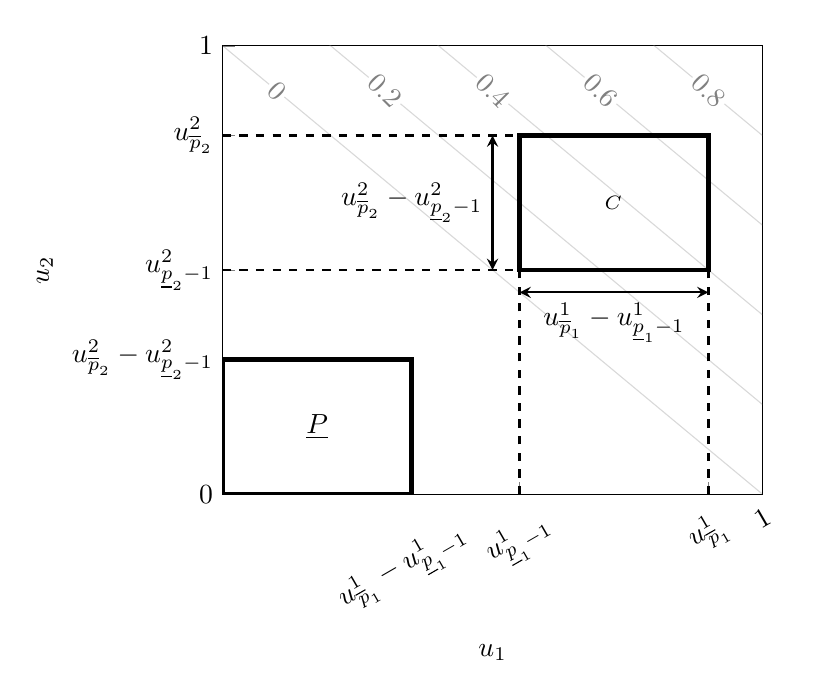
\begin{tikzpicture}
        \begin{axis}[%
            xlabel=$u_1$,
            ylabel=$u_2$,
            xmin=0, xmax=1,
            ymin=0, ymax=1,
            xtick={0.35, 0.55,  0.9, 1},
            xticklabels={$u^1_{\overline{p}_1} - u^1_{\underline{p}_1-1}~~$, $u^1_{\underline{p}_1-1}$, $u^1_{\overline{p}_1}$, $1$},
            ytick={0, 0.3, 0.5,  0.8, 1},
            yticklabels={$0$, $u^2_{\overline{p}_2} - u^2_{\underline{p}_2-1}$, $u^2_{\underline{p}_2-1}$, $u^2_{\overline{p}_2}$, $1$},
            xticklabel style={rotate=30},
            xtick pos=left,
            ytick pos=left,],
            
            \addplot [domain=0:1,samples=40,draw opacity=0.3,color=gray]({x},{1-x});
            \addplot [domain=0:1,samples=40,draw opacity=0.3,color=gray]({x},{1.2-x}); 
            \addplot [domain=0:1,samples=40,draw opacity=0.3,color=gray]({x},{1.4-x}); 
            \addplot [domain=0:1,samples=40,draw opacity=0.3,color=gray]({x},{1.6-x}); 
            \addplot [domain=0:1,samples=40,draw opacity=0.3,color=gray]({x},{1.8-x});

            \node[rotate=-45, fill=white, rounded corners=2pt, inner sep=1pt] (x) at (0.1, 0.9) {\color{gray}0};
            \node[rotate=-45, fill=white, rounded corners=2pt, inner sep=1pt] (x) at (0.3, 0.9) {\color{gray}0.2};
            \node[rotate=-45, fill=white, rounded corners=2pt, inner sep=1pt] (x) at (0.5, 0.9) {\color{gray}0.4};
            \node[rotate=-45, fill=white, rounded corners=2pt, inner sep=1pt] (x) at (0.7, 0.9) {\color{gray}0.6};
            \node[rotate=-45, fill=white, rounded corners=2pt, inner sep=1pt] (x) at (0.9, 0.9) {\color{gray}0.8};
            
            
            \node (a) at (0.9, 0.8) {};
            \node (b) at (0.55, 0.8) {};
            \node (c) at (0.55, 0.5) {};
            \node (d) at (0.9, 0.5) {};
            \draw[ultra thick, black] (c.center) rectangle (a.center) node[pos=0.5]{$\Bel_C$};
            
            \node (e) at (0, 0.8) {};
            \node (f) at (0, 0.5) {};
            \node (g) at (0.9, 0) {};
            \node (h) at (0.55, 0) {};
            \draw[thick, dashed, black] (e.center) -- (b.center);
            \draw[thick, dashed, black] (f.center) -- (c.center);
            \draw[thick, dashed, black] (g.center) -- (d.center);
            \draw[thick, dashed, black] (h.center) -- (c.center);
            
            \node (i) at (0.35, 0.3) {};
            \node (j) at (0, 0) {};
            \draw[ultra thick, black] (i.center) rectangle (j.center) node[pos=0.5]{$\underline{P}$};
            
            \node (m) at (0.55, 0.45) {};
            \node (n) at (0.9, 0.45) {};
            \node (o) at (0.5, 0.8) {};
            \node (p) at (0.5, 0.5) {};
            \draw [stealth-stealth, thick, black] (m.center) -- (n.center) node[pos=0.5, below]{$u^1_{\overline{p}_1} - u^1_{\underline{p}_1-1}$};
            \draw [stealth-stealth, thick, black] (o.center) -- (p.center) node[pos=0.5, left]{$u^2_{\overline{p}_2} - u^2_{\underline{p}_2-1}$};
        
        \end{axis}
    \end{tikzpicture}
    \caption{Bird's-eye view of the \L ukaciewicz 2-copula $C_L$, where the gray lines are the isolines of the copula. $\Bel_C$ and $\underline{P}$ are represented in the case where the marginals are p-boxes. The thick rectangles represent the bounds on which to compute the H-volume. Numbers $u^i_k$ use the notation of the proof of \Cref{prop:convexity_pbox}.}
    \label{fig:copula_convex}
 
\end{figure}
\section{Consistency of the Median Filtering}\label{sec:median_filtering}
This section demonstrates a result used in \Cref{sec:coherence_disparity_intervals}. We define the median of a set of $n$ sorted values $X=\{x_1\enum x_n\}$ is defined as
    \begin{align}
        &\text{if }n=2l+1,\qquad \median X =& x_{l+1}\\
        &\text{if }n=2l,\qquad \median X =& \frac{x_{l}+x_{l+1}}{2}
    \end{align}
    where $l$ is an integer.

\begin{proposition}\label{prop:median_consistency}
    Let $n\in\mathbb{N}^*$. Let $X=\{x_1\enum x_n\}$ and $Y=\{y_1\enum y_n\}$ be two sets of integers such that for all $i$ in $\opi1,n\cli$, $x_i\leqslant y_i$. Then:
    \begin{align}
        \median X \leqslant \median Y
    \end{align}
\end{proposition}

\begin{proof}
    Let $\sigma_X:\opi1,n\cli\rightarrow\opi1,n\cli$ be a bijection sorting $X$, \ie:
    \begin{align}
        x_{\sigma_X(1)}\leqslant\dots\leqslant x_{\sigma_X(i)}\leqslant\dots\leqslant x_{\sigma_X(n)}
    \end{align}
    We define $\sigma_Y:\opi1,n\cli\rightarrow\opi1,n\cli$ similarly, this time sorting $Y$. Notice that it does not necessarily holds that $x_{\sigma_X(i)}\leqslant y_{\sigma_Y(i)}$, but only that $x_{\sigma_Y(i)}\leqslant y_{\sigma_Y(i)}$ 
    
    Suppose that $n=2l+1$ where $l$ is an integer. Then the median of $X$ equals $x_{\sigma_X(l+1)}$ and the median of $Y$ equals $y_{\sigma_Y(l+1)}$ 
    It holds that for all $i\in\opi1,l+1\cli$:
    \begin{align}
        y_{\sigma_Y(l+1)}\geqslant y_{\sigma_Y(i)}\geqslant x_{\sigma_Y(i)}
    \end{align}
    The median of $Y$ is thus greater than at least $l+1$ elements of $X$. Because the $(l+1)$\ith smallest element of $X$ is the median of $X$, then the median of $Y$ is necessarily greater than the median of $X$.
    
    The case $n=2l$, is somehow similar. With the same arguments, we can say that $y_{\sigma_Y(l+1)}$ is greater than $l+1$ elements of $X$, thus it is greater than its $(l+1)$\ith smallest element $x_{\sigma_X(l+1)}$. Similarly, $y_{\sigma_Y(l)}$ is greater than $l$ elements of $X$, thus it is greater than its $l$\ith smallest element $x_{\sigma_X(l)}$. Therefore, it holds that:
    \begin{align}
        \frac{y_{\sigma_Y(l)}+y_{\sigma_Y(l+1)}}{2}\geqslant\frac{x_{\sigma_X(l)}+x_{\sigma_X(l+1)}}{2}
    \end{align}
    Which also means that the median of $Y$ is necessarily greater than the median of $X$.
\end{proof}

\section{Ablation Studies for Disparity Confidence Intervals}\label{sec:ablation_study}
This section will present ablation studies regarding the different parameters used to create disparity confidence intervals in \Cref{chap:epistemic_uncertainty}. When not specified, the values of the different parameters are fixed to the same values used in our experiments, \ie:\newline\medskip
\begin{minipage}{0.5\linewidth}
\begin{align*}
    &\alpha = 0.9\\
    &\tau_{amb} = 0.6\\
    &n_\N = 2
\end{align*}
\end{minipage}
\begin{minipage}{0.5\linewidth}
\begin{align*}
    &q = 0.9\\
    &k_{amb} = 2\\
\end{align*}
\end{minipage}\bigskip\newline
Those values were determined by evaluating different metrics on specific scenes of the Middlebury dataset. We present some results on the Middlebury Cones stereo images. In our experiments, we used the same values of parameters for every scene and for the two considered cost functions: CENSUS and MC-CNN. More in-depth analyses could lead to sets of parameter values specialized for each cost function. This is left as future work, considering that only the CENSUS cost function is used in \Cref{chap:elevation_intervals}.

\subsection{Possibility Threshold}
In \Cref{eq:set_of_possible_disparities}, we considered a parameter $\alpha$ used as a possibility threshold to compute a set of most possible disparities. We recall here the equations used in this section to compute confidence intervals:
\begin{align*}
    D_\alpha&=\{~ d ~|~ \pi_{\rowcol}(d)\geqslant\alpha\}\\
    I_\alpha &= [\underline{I}_\alpha,~\overline{I}_\alpha]=[\min D_\alpha, ~\max D_\alpha]
\end{align*}

Higher values of $\alpha$ will lead to smaller disparity sets, and thus to smaller intervals. In \Cref{chap:epistemic_uncertainty,chap:elevation_intervals}, we chose to use $\alpha=0.9$, but other values could be considered. \Cref{fig:ablation_study_alpha_1,fig:ablation_study_alpha_2} presents the evolution of metrics for different values of $\alpha$. As expected, the accuracy decreases with higher values of $\alpha$, as displayed in \Cref{fig:ablation_study_alpha_acc}.

\Cref{fig:ablation_study_alpha_eps} displays the influence of $\alpha$ over the residual error $\varepsilon$. Variations of $\varepsilon$ have a magnitude of around $2\%$, which indicates that $\alpha$ has very little influence over this metric. $\varepsilon$ is not monotone with regard to $\alpha$. This can be explained as follows: as $\alpha$ increases, the size of intervals decreases. There are thus more intervals that do not contain the ground truth, effectively modifying the set for which $\varepsilon$ is the median. There is therefore no guarantee that $\epsilon$ is monotone with regard to $\alpha$. 

\Cref{fig:ablation_study_alpha_s_rel} displays the influence of $\alpha$ over the relative size $s_{rel}$ of intervals in high confidence areas. $\alpha$ does not have an influence over $s_{rel}$ for the CENSUS cost function, and small influence for the MC-CNN cost function (fluctuations of $3\%$ only). 

In \Cref{fig:ablation_study_alpha_o_rel}, we can observe that the relative over-estimation also decreases with higher values of $\alpha$. For the CENSUS cost function, the relative over-estimation $o_{rel}$ decreases less rapidly for values $\alpha\geqslant0.9$. $\alpha=0.9$ ensures that the relative over-estimation is less than $50\%$ for both cost functions, which we consider a satisfying size for intervals in low confidence areas. 
\begin{figure}
    \centering
    \begin{subfigure}[t]{0.7\linewidth}
        \centering
        \includegraphics[width=\linewidth]{Images/X_Annex/ablation_study_cones_alpha_acc.png}
        \caption{Accuracy $acc$ for different values of the parameter $\alpha$ for constructing intervals.}
        \label{fig:ablation_study_alpha_acc}
    \end{subfigure}\vspace*{0.3cm}\\
    \begin{subfigure}[t]{0.7\linewidth}
        \centering
        \includegraphics[width=\linewidth]{Images/X_Annex/ablation_study_cones_alpha_eps.png}
        \caption{Residual error $\varepsilon$ for different values of the parameter $\alpha$ for constructing intervals.}
        \label{fig:ablation_study_alpha_eps}
    \end{subfigure}
    \caption{Influence of the parameter $\alpha$ used for constructing intervals in \Cref{eq:set_of_possible_disparities} for Middlebury Cones stereo images. Intervals were regularized in low confidence areas.}
    \label{fig:ablation_study_alpha_1}
\end{figure}
\begin{figure}
    \centering
    \begin{subfigure}[t]{0.7\linewidth}
        \centering
        \includegraphics[width=\linewidth]{Images/X_Annex/ablation_study_cones_alpha_s_rel.png}
        \caption{Relative size $s_{rel}$ for different values of the parameter $\alpha$ for constructing intervals.}
        \label{fig:ablation_study_alpha_s_rel}
    \end{subfigure}\vspace*{0.3cm}\\
    \begin{subfigure}[t]{0.7\linewidth}
        \centering
        \includegraphics[width=\linewidth]{Images/X_Annex/ablation_study_cones_alpha_o_rel.png}
        \caption{Relative over-estimation $o_rel$ for different values of the parameter $\alpha$ for constructing intervals.}
        \label{fig:ablation_study_alpha_o_rel}
    \end{subfigure}
    \caption{Influence of the parameter $\alpha$ used for constructing intervals in \Cref{eq:set_of_possible_disparities} for Middlebury Cones stereo images. Intervals were regularized in low confidence areas.}
    \label{fig:ablation_study_alpha_2}
\end{figure}

\subsection{Low Confidence Areas}
In \Cref{chap:epistemic_uncertainty}, we noticed that intervals that did not contain the ground truth were usually located in low confidence areas. We thus proposed to detect low confidence areas in order to process the intervals differently there. We recall \Cref{eq:low_confidence_area,eq:n_N} used to define low confidence areas. A pixel $(\rowcol)$ is considered to be in a low confidence area if it verifies:
\begin{align*}
    \min c_{amb}(\rowcol+k)=\min_{-k_{amb}~\leqslant~ k~\leqslant ~k_{amb}}c_{amb}(\rowcol+k)\leqslant \tau_{amb}
\end{align*}
This equation translates the fact that we use a minitive kernel to filter the confidence from ambiguity map, of size $(1, 2\times k_{amb}+1)$. High values of $k_{amb}$ lead to lower values of the confidence from ambiguity, and consequently to more low confidence pixels. Similarly, higher values of the threshold $\tau_{amb}$ lead to more low confidence pixels. In \Cref{sec:regularization_of_intervals}, we also considered low confidence neighboring $\N(\rowcol)$ of a low confidence pixel, defined as:
\begin{align*}
    \N(row,~col) = \{ p\in &\bigcup_{-n_\N\leqslant k\leqslant n_\N}S(row+k, ~col_k)\\
    &\st~S(row + (k+1), ~col_{k+1})\text{ is adjacent to }S(row+k, ~col_{k})\}
\end{align*}
where $S$ is defined as:
\begin{align*}
    S(\rowcol) = \{~ (row,~col') \text{ \st }~\forall c\in\opi col, col'\cli,~\min c_{amb}(row, ~c+k)\leqslant \tau_{amb}~\}
\end{align*}
Given a low confidence pixel $(\rowcol)$, the parameter $n_\N$ defines the number of rows above and below a pixel that will be explored when defining its neighboring. High values of $n_\N$ will lead to neighboring with more low confidence pixels, but does not influence the total amount of low confidence pixels present in an image.

In \Cref{chap:epistemic_uncertainty,chap:elevation_intervals}, we chose to use $\tau_{amb}=0.6$, $k_{amb}=2$ and $n_\N=2$. We detail here the influence of those parameters.

We want low confidence areas to include as many wrong intervals as possible, but they should not be covering the entire image either. We also want to consider true intervals in the low confidence areas so that our quantile regularization is based on a sufficient pool of correct intervals. For this reason, computing the F1-score is not relevant. We therefore consider two metrics separately: the coverage and the proportion of low confidence pixels. The coverage is the proportion of wrong intervals that are also low confidence pixels:
\begin{align*}
    \mathrm{Coverage} = \dfrac{\#\{(\rowcol)~\st~d_{true}\not\in I_\alpha\text{ and }\min c_{amb}(\rowcol+k)\leqslant \tau_{amb} \}}{\#\{\rowcol)~\st~d_{true}\not\in I_\alpha\}}
\end{align*}
The proportion of low confidence pixels is simply the proportion of low confidence pixels in the entire left image.
\Cref{fig:ablation_study_tau_coverage,fig:ablation_study_tau_size} respectively display the evolution of the coverage and of the proportion of low confidence pixels for different values of $\tau_{amb}$. \Cref{fig:ablation_study_k_coverage,fig:ablation_study_k_size} display the same metrics, but for different values of $k_{amb}$. We can see that the value $\tau_{amb}=0.6$ guarantees a coverage superior to $60\%$ while maintaining a proportion of low confidence pixels smaller than $20\%$ in the case of Middlebury Cones, for both considered cost functions. Similarly, $k_{amb}=2$ guarantees a coverage superior to $60\%$ while maintaining a proportion of low confidence pixels smaller than $20\%$ in the case of Middlebury Cones, for both considered cost functions. In general, the coverage and proportion of low confidence pixels are more sensitive to a variation of $0.1$ of $\tau_{amb}$ than a variation of $1$ of the kernel size parameter $k_{amb}$.

\begin{figure}
    \centering
    \begin{subfigure}[t]{0.7\linewidth}
        \centering
        \includegraphics[width=\linewidth]{Images/X_Annex/ablation_study_cones_tau_amb.png}
        \caption{Coverage for different values of the parameter $\tau_{amb}$ for detecting wrong intervals in low confidence areas.}
        \label{fig:ablation_study_tau_coverage}
    \end{subfigure}\vspace*{0.3cm}\\
    \begin{subfigure}[t]{0.7\linewidth}
        \centering
        \includegraphics[width=\linewidth]{Images/X_Annex/ablation_study_cones_tau_amb_2.png}
        \caption{Proportion of pixels detected as low confidence pixels depending on the value $\tau_{amb}$}
        \label{fig:ablation_study_tau_size}
    \end{subfigure}
    \caption{Influence of the parameter $\tau_{amb}$ used for interval regularization in \Cref{eq:low_confidence_area} for Middlebury Cones stereo images.}
    \label{fig:ablation_study_tau}
\end{figure}

\begin{figure}
    \centering
    \begin{subfigure}[t]{0.7\linewidth}
        \centering
        \includegraphics[width=\linewidth]{Images/X_Annex/ablation_study_cones_k_amb.png}
        \caption{Coverage for different values of the parameter $k_{amb}$ for detecting wrong intervals in low confidence areas.}
        \label{fig:ablation_study_k_coverage}
    \end{subfigure}\vspace*{0.3cm}\\
    \begin{subfigure}[t]{0.7\linewidth}
        \centering
        \includegraphics[width=\linewidth]{Images/X_Annex/ablation_study_cones_k_amb_2.png}
        \caption{Proportion of pixels detected as low confidence pixels depending on the value $k_{amb}$}
        \label{fig:ablation_study_k_size}
    \end{subfigure}
    \caption{Influence of the parameter $k_{amb}$ used for interval regularization in \Cref{eq:low_confidence_area} for Middlebury Cones stereo images.}
    \label{fig:ablation_study_k}
\end{figure}

\Cref{fig:ablation_study_n_N} displays the influence of $n_\N$ over the accuracy, and over the number of pixels in low confidence neighboring $n_\N$. \Cref{fig:ablation_study_n_N_acc} shows that $n_\N$ increases the global accuracy, but it is less sensitive to variations of $n_\N$ than it is to variation of $\alpha$ from \Cref{fig:ablation_study_alpha_acc}. \Cref{fig:ablation_study_n_N_hist_1,fig:ablation_study_n_N_hist_2} shows that $n_\N\geqslant2$ strongly reduces the number of low confidence neighboring with less than $50$ pixels. However, high values of $n_\N$ increases the computation complexity for a small gain of accuracy. We therefore choose $n_\N=2$ as a trade-off.

\begin{figure}
    \centering
    \begin{subfigure}[t]{0.7\linewidth}
        \centering
        \includegraphics[width=\linewidth]{Images/X_Annex/ablation_study_cones_n_N_1.png}
        \caption{Accuracy $acc$ for different values of $n_\N$}
        \label{fig:ablation_study_n_N_acc}
    \end{subfigure}\vspace*{0.3cm}\\
    \begin{subfigure}[t]{0.7\linewidth}
        \centering
        \includegraphics[width=\linewidth]{Images/X_Annex/ablation_study_cones_n_N_2.png}
        \caption{Histograms of the number of pixels in low confidence areas $\N(\rowcol)$ for $n_\N\in\{1,2,3\}$.}
        \label{fig:ablation_study_n_N_hist_1}
    \end{subfigure}\vspace*{0.3cm}\\
    \begin{subfigure}[t]{0.7\linewidth}
        \centering
        \includegraphics[width=\linewidth]{Images/X_Annex/ablation_study_cones_n_N_3.png}
        \caption{Histograms of the number of pixels in low confidence areas $\N(\rowcol)$ for $n_\N\in\{4,5,6\}$.} 
        \label{fig:ablation_study_n_N_hist_2}
    \end{subfigure}
    \caption{Influence of the parameter $n_\N$ used for interval regularization in \Cref{eq:n_N} using the CENSUS cost function on Middlebury cones.}
    \label{fig:ablation_study_n_N}
\end{figure}

\subsection{Quantile Regularization}
Once the neighboring $\N$ of a low confidence pixel has been computed, we update the value of its confidence interval based on the distributions of intervals of its neighbors. We recall here \Cref{eq:quantile_reg} used for the regularization of intervals:
\begin{align*}
    I^{reg}_\alpha=[&\mathcal{Q}_{1-q}(\{\underline{I}_\alpha(r,~c)~|~(r,~c)\in\N(\rowcol)\}),\nonumber\\
    &\mathcal{Q}_q(\{\overline{I}_\alpha(r,~c)~|~(r,~c)\in\N(\rowcol)\})]
\end{align*}
where $\mathcal{Q}_q$ refers to the $q$\ith quantile of a set. In our experiments, we used $q=0.9$.

\begin{figure}
    \centering
    \begin{subfigure}[t]{0.7\linewidth}
        \centering
        \includegraphics[width=\linewidth]{Images/X_Annex/ablation_study_cones_q_acc.png}
        \caption{Accuracy $acc$ with regularization for different quantiles $q$}
        \label{fig:ablation_study_q_no_reg}
    \end{subfigure}\vspace*{0.3cm}\\
    \begin{subfigure}[t]{0.7\linewidth}
        \centering
        \includegraphics[width=\linewidth]{Images/X_Annex/ablation_study_cones_q_o_rel.png}
        \caption{Relative over-estimation $o_{rel}$ with regularization for different quantiles $q$}
        \label{fig:ablation_study_q_reg}
    \end{subfigure}
    \caption{Influence of the parameter $q$ used for interval regularization in \Cref{eq:quantile_reg} for Middlebury Cones stereo images.}
    \label{fig:ablation_study_q}
\end{figure}

\Cref{fig:ablation_study_q} displays the influence of the parameter $q$ over the accuracy and relative over-estimation for the Middlebury Cones stereo images. As expected, both the accuracy and relative over-estimation increase with the value of $q$.

\begin{figure}
    \begin{subfigure}[t]{0.5\linewidth}
        \flushleft
        \includegraphics[width=\linewidth]{Images/X_Annex/ablation_study_acc_reg_no_reg_CENSUS.png}
        \caption{CENSUS cost function}
        \label{fig:acc_no_reg_CENSUS}
    \end{subfigure}
    \begin{subfigure}[t]{0.5\linewidth}
        \flushright
        \includegraphics[width=\linewidth]{Images/X_Annex/ablation_study_acc_reg_no_reg_MCCNN.png}
        \caption{MC-CNN cost function}
        \label{fig:acc_no_reg_MCCNN}
    \end{subfigure}
    \caption{Accuracy with and without regularization of intervals in low confidence areas for different scenes of the Middlebury dataset.}
    \label{fig:acc_reg_no_reg}
\end{figure}

\Cref{fig:acc_reg_no_reg} displays the accuracy with and without regularization for scenes of the Middlebury dataset. Without the regularization, many scenes do not reach an accuracy of $90\%$. This is especially true for the CENSUS cost function. This justifies the use of the regularization step from \Cref{sec:regularization_of_intervals}.

\clearpage